% Generated by Sphinx.
\def\sphinxdocclass{report}
\documentclass[letterpaper,10pt,english]{sphinxmanual}
\usepackage[utf8]{inputenc}
\DeclareUnicodeCharacter{00A0}{\nobreakspace}
\usepackage{cmap}
\usepackage[T1]{fontenc}
\usepackage{babel}
\usepackage{times}
\usepackage[Bjarne]{fncychap}
\usepackage{longtable}
\usepackage{sphinx}
\usepackage{multirow}

\addto\captionsenglish{\renewcommand{\figurename}{Fig. }}
\addto\captionsenglish{\renewcommand{\tablename}{Table }}
\floatname{literal-block}{Listing }



\title{nidm Documentation}
\date{October 30, 2015}
\release{1.0}
\author{NIDASH Working Group}
\newcommand{\sphinxlogo}{}
\renewcommand{\releasename}{Release}
\makeindex

\makeatletter
\def\PYG@reset{\let\PYG@it=\relax \let\PYG@bf=\relax%
    \let\PYG@ul=\relax \let\PYG@tc=\relax%
    \let\PYG@bc=\relax \let\PYG@ff=\relax}
\def\PYG@tok#1{\csname PYG@tok@#1\endcsname}
\def\PYG@toks#1+{\ifx\relax#1\empty\else%
    \PYG@tok{#1}\expandafter\PYG@toks\fi}
\def\PYG@do#1{\PYG@bc{\PYG@tc{\PYG@ul{%
    \PYG@it{\PYG@bf{\PYG@ff{#1}}}}}}}
\def\PYG#1#2{\PYG@reset\PYG@toks#1+\relax+\PYG@do{#2}}

\expandafter\def\csname PYG@tok@gd\endcsname{\def\PYG@tc##1{\textcolor[rgb]{0.63,0.00,0.00}{##1}}}
\expandafter\def\csname PYG@tok@gu\endcsname{\let\PYG@bf=\textbf\def\PYG@tc##1{\textcolor[rgb]{0.50,0.00,0.50}{##1}}}
\expandafter\def\csname PYG@tok@gt\endcsname{\def\PYG@tc##1{\textcolor[rgb]{0.00,0.27,0.87}{##1}}}
\expandafter\def\csname PYG@tok@gs\endcsname{\let\PYG@bf=\textbf}
\expandafter\def\csname PYG@tok@gr\endcsname{\def\PYG@tc##1{\textcolor[rgb]{1.00,0.00,0.00}{##1}}}
\expandafter\def\csname PYG@tok@cm\endcsname{\let\PYG@it=\textit\def\PYG@tc##1{\textcolor[rgb]{0.25,0.50,0.56}{##1}}}
\expandafter\def\csname PYG@tok@vg\endcsname{\def\PYG@tc##1{\textcolor[rgb]{0.73,0.38,0.84}{##1}}}
\expandafter\def\csname PYG@tok@m\endcsname{\def\PYG@tc##1{\textcolor[rgb]{0.13,0.50,0.31}{##1}}}
\expandafter\def\csname PYG@tok@mh\endcsname{\def\PYG@tc##1{\textcolor[rgb]{0.13,0.50,0.31}{##1}}}
\expandafter\def\csname PYG@tok@cs\endcsname{\def\PYG@tc##1{\textcolor[rgb]{0.25,0.50,0.56}{##1}}\def\PYG@bc##1{\setlength{\fboxsep}{0pt}\colorbox[rgb]{1.00,0.94,0.94}{\strut ##1}}}
\expandafter\def\csname PYG@tok@ge\endcsname{\let\PYG@it=\textit}
\expandafter\def\csname PYG@tok@vc\endcsname{\def\PYG@tc##1{\textcolor[rgb]{0.73,0.38,0.84}{##1}}}
\expandafter\def\csname PYG@tok@il\endcsname{\def\PYG@tc##1{\textcolor[rgb]{0.13,0.50,0.31}{##1}}}
\expandafter\def\csname PYG@tok@go\endcsname{\def\PYG@tc##1{\textcolor[rgb]{0.20,0.20,0.20}{##1}}}
\expandafter\def\csname PYG@tok@cp\endcsname{\def\PYG@tc##1{\textcolor[rgb]{0.00,0.44,0.13}{##1}}}
\expandafter\def\csname PYG@tok@gi\endcsname{\def\PYG@tc##1{\textcolor[rgb]{0.00,0.63,0.00}{##1}}}
\expandafter\def\csname PYG@tok@gh\endcsname{\let\PYG@bf=\textbf\def\PYG@tc##1{\textcolor[rgb]{0.00,0.00,0.50}{##1}}}
\expandafter\def\csname PYG@tok@ni\endcsname{\let\PYG@bf=\textbf\def\PYG@tc##1{\textcolor[rgb]{0.84,0.33,0.22}{##1}}}
\expandafter\def\csname PYG@tok@nl\endcsname{\let\PYG@bf=\textbf\def\PYG@tc##1{\textcolor[rgb]{0.00,0.13,0.44}{##1}}}
\expandafter\def\csname PYG@tok@nn\endcsname{\let\PYG@bf=\textbf\def\PYG@tc##1{\textcolor[rgb]{0.05,0.52,0.71}{##1}}}
\expandafter\def\csname PYG@tok@no\endcsname{\def\PYG@tc##1{\textcolor[rgb]{0.38,0.68,0.84}{##1}}}
\expandafter\def\csname PYG@tok@na\endcsname{\def\PYG@tc##1{\textcolor[rgb]{0.25,0.44,0.63}{##1}}}
\expandafter\def\csname PYG@tok@nb\endcsname{\def\PYG@tc##1{\textcolor[rgb]{0.00,0.44,0.13}{##1}}}
\expandafter\def\csname PYG@tok@nc\endcsname{\let\PYG@bf=\textbf\def\PYG@tc##1{\textcolor[rgb]{0.05,0.52,0.71}{##1}}}
\expandafter\def\csname PYG@tok@nd\endcsname{\let\PYG@bf=\textbf\def\PYG@tc##1{\textcolor[rgb]{0.33,0.33,0.33}{##1}}}
\expandafter\def\csname PYG@tok@ne\endcsname{\def\PYG@tc##1{\textcolor[rgb]{0.00,0.44,0.13}{##1}}}
\expandafter\def\csname PYG@tok@nf\endcsname{\def\PYG@tc##1{\textcolor[rgb]{0.02,0.16,0.49}{##1}}}
\expandafter\def\csname PYG@tok@si\endcsname{\let\PYG@it=\textit\def\PYG@tc##1{\textcolor[rgb]{0.44,0.63,0.82}{##1}}}
\expandafter\def\csname PYG@tok@s2\endcsname{\def\PYG@tc##1{\textcolor[rgb]{0.25,0.44,0.63}{##1}}}
\expandafter\def\csname PYG@tok@vi\endcsname{\def\PYG@tc##1{\textcolor[rgb]{0.73,0.38,0.84}{##1}}}
\expandafter\def\csname PYG@tok@nt\endcsname{\let\PYG@bf=\textbf\def\PYG@tc##1{\textcolor[rgb]{0.02,0.16,0.45}{##1}}}
\expandafter\def\csname PYG@tok@nv\endcsname{\def\PYG@tc##1{\textcolor[rgb]{0.73,0.38,0.84}{##1}}}
\expandafter\def\csname PYG@tok@s1\endcsname{\def\PYG@tc##1{\textcolor[rgb]{0.25,0.44,0.63}{##1}}}
\expandafter\def\csname PYG@tok@gp\endcsname{\let\PYG@bf=\textbf\def\PYG@tc##1{\textcolor[rgb]{0.78,0.36,0.04}{##1}}}
\expandafter\def\csname PYG@tok@sh\endcsname{\def\PYG@tc##1{\textcolor[rgb]{0.25,0.44,0.63}{##1}}}
\expandafter\def\csname PYG@tok@ow\endcsname{\let\PYG@bf=\textbf\def\PYG@tc##1{\textcolor[rgb]{0.00,0.44,0.13}{##1}}}
\expandafter\def\csname PYG@tok@sx\endcsname{\def\PYG@tc##1{\textcolor[rgb]{0.78,0.36,0.04}{##1}}}
\expandafter\def\csname PYG@tok@bp\endcsname{\def\PYG@tc##1{\textcolor[rgb]{0.00,0.44,0.13}{##1}}}
\expandafter\def\csname PYG@tok@c1\endcsname{\let\PYG@it=\textit\def\PYG@tc##1{\textcolor[rgb]{0.25,0.50,0.56}{##1}}}
\expandafter\def\csname PYG@tok@kc\endcsname{\let\PYG@bf=\textbf\def\PYG@tc##1{\textcolor[rgb]{0.00,0.44,0.13}{##1}}}
\expandafter\def\csname PYG@tok@c\endcsname{\let\PYG@it=\textit\def\PYG@tc##1{\textcolor[rgb]{0.25,0.50,0.56}{##1}}}
\expandafter\def\csname PYG@tok@mf\endcsname{\def\PYG@tc##1{\textcolor[rgb]{0.13,0.50,0.31}{##1}}}
\expandafter\def\csname PYG@tok@err\endcsname{\def\PYG@bc##1{\setlength{\fboxsep}{0pt}\fcolorbox[rgb]{1.00,0.00,0.00}{1,1,1}{\strut ##1}}}
\expandafter\def\csname PYG@tok@mb\endcsname{\def\PYG@tc##1{\textcolor[rgb]{0.13,0.50,0.31}{##1}}}
\expandafter\def\csname PYG@tok@ss\endcsname{\def\PYG@tc##1{\textcolor[rgb]{0.32,0.47,0.09}{##1}}}
\expandafter\def\csname PYG@tok@sr\endcsname{\def\PYG@tc##1{\textcolor[rgb]{0.14,0.33,0.53}{##1}}}
\expandafter\def\csname PYG@tok@mo\endcsname{\def\PYG@tc##1{\textcolor[rgb]{0.13,0.50,0.31}{##1}}}
\expandafter\def\csname PYG@tok@kd\endcsname{\let\PYG@bf=\textbf\def\PYG@tc##1{\textcolor[rgb]{0.00,0.44,0.13}{##1}}}
\expandafter\def\csname PYG@tok@mi\endcsname{\def\PYG@tc##1{\textcolor[rgb]{0.13,0.50,0.31}{##1}}}
\expandafter\def\csname PYG@tok@kn\endcsname{\let\PYG@bf=\textbf\def\PYG@tc##1{\textcolor[rgb]{0.00,0.44,0.13}{##1}}}
\expandafter\def\csname PYG@tok@o\endcsname{\def\PYG@tc##1{\textcolor[rgb]{0.40,0.40,0.40}{##1}}}
\expandafter\def\csname PYG@tok@kr\endcsname{\let\PYG@bf=\textbf\def\PYG@tc##1{\textcolor[rgb]{0.00,0.44,0.13}{##1}}}
\expandafter\def\csname PYG@tok@s\endcsname{\def\PYG@tc##1{\textcolor[rgb]{0.25,0.44,0.63}{##1}}}
\expandafter\def\csname PYG@tok@kp\endcsname{\def\PYG@tc##1{\textcolor[rgb]{0.00,0.44,0.13}{##1}}}
\expandafter\def\csname PYG@tok@w\endcsname{\def\PYG@tc##1{\textcolor[rgb]{0.73,0.73,0.73}{##1}}}
\expandafter\def\csname PYG@tok@kt\endcsname{\def\PYG@tc##1{\textcolor[rgb]{0.56,0.13,0.00}{##1}}}
\expandafter\def\csname PYG@tok@sc\endcsname{\def\PYG@tc##1{\textcolor[rgb]{0.25,0.44,0.63}{##1}}}
\expandafter\def\csname PYG@tok@sb\endcsname{\def\PYG@tc##1{\textcolor[rgb]{0.25,0.44,0.63}{##1}}}
\expandafter\def\csname PYG@tok@k\endcsname{\let\PYG@bf=\textbf\def\PYG@tc##1{\textcolor[rgb]{0.00,0.44,0.13}{##1}}}
\expandafter\def\csname PYG@tok@se\endcsname{\let\PYG@bf=\textbf\def\PYG@tc##1{\textcolor[rgb]{0.25,0.44,0.63}{##1}}}
\expandafter\def\csname PYG@tok@sd\endcsname{\let\PYG@it=\textit\def\PYG@tc##1{\textcolor[rgb]{0.25,0.44,0.63}{##1}}}

\def\PYGZbs{\char`\\}
\def\PYGZus{\char`\_}
\def\PYGZob{\char`\{}
\def\PYGZcb{\char`\}}
\def\PYGZca{\char`\^}
\def\PYGZam{\char`\&}
\def\PYGZlt{\char`\<}
\def\PYGZgt{\char`\>}
\def\PYGZsh{\char`\#}
\def\PYGZpc{\char`\%}
\def\PYGZdl{\char`\$}
\def\PYGZhy{\char`\-}
\def\PYGZsq{\char`\'}
\def\PYGZdq{\char`\"}
\def\PYGZti{\char`\~}
% for compatibility with earlier versions
\def\PYGZat{@}
\def\PYGZlb{[}
\def\PYGZrb{]}
\makeatother

\renewcommand\PYGZsq{\textquotesingle}

\begin{document}

\maketitle
\tableofcontents
\phantomsection\label{index::doc}


This is a tool to deploy a REST API to run queries on and visualize NIDM turtle objects. Queries can be found in the \href{https://github.com/incf-nidash/nidm-query}{nidm-query}, repo, along with a \href{https://github.com/vsoch/nidmviewer}{nidm viewer}.  This API is under development, and please submit issues and requests to the \href{https://github.com/incf-nidash/nidm-api/issues}{nidm-api} repo.


\chapter{Why do I want to use this?}
\label{index:nidm-api}\label{index:why-do-i-want-to-use-this}
You might want to use this tool if you have a NIDM data structure, meaning NIDM-results, NIDM-experiment, or NIDM-workflow, and you want to get information out of it but you don't know a single thing about RDF files or the query language for them, which is called sparql. This tool will allow you to run pre-generated queries easily, and return results in a format that is easily parsable by modern web technologies (eg, json for javascript or python), and (coming soon) csv and tsv files.


\chapter{Under Development}
\label{index:under-development}
The tool currently implements returning basic json from a query against a ttl (turtle) file. The following will be developed:
\begin{itemize}
\item {} 
interactive interfaces for creating new queries

\item {} 
returning interactive graphs (d3, neo4j)

\item {} 
functions to search / filter queries

\item {} 
returning more data types

\item {} 
validation of query data structures

\end{itemize}

Contents:


\section{Installation}
\label{installation:installation}\label{installation::doc}
To install

\begin{Verbatim}[commandchars=\\\{\}]
pip install git+git://github.com/incf\PYGZhy{}nidash/nidm\PYGZhy{}api.git
\end{Verbatim}


\section{Getting Started}
\label{getting-started:getting-started}\label{getting-started::doc}
You have three options for using the nidm-api: as a local REST API, a REST API (served to the world on a public server), or as modules (to integrate into your python applications).


\subsection{Local Machine REST API}
\label{getting-started:local-machine-rest-api}
When you install the module, an executable, ``nidm'' is placed into your system or local bin (it will tell you the location upon installation). If this bin is added to your path, you can start the server:

\begin{Verbatim}[commandchars=\\\{\}]
\PYG{n}{nidm}
\end{Verbatim}

Then open your browser to localhost:8088. The index view that you see is a complete list of validated queries, for example:

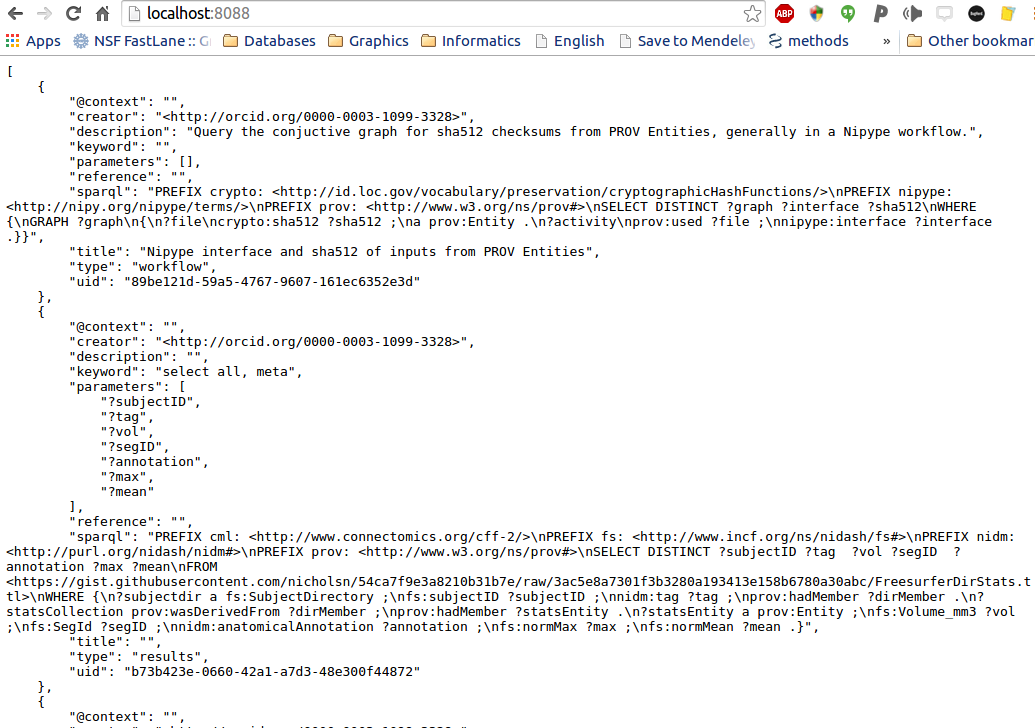
\includegraphics{apiQueryMeta.png}

The available queries must pass through validation to be available (not yet implemented). The queries are organized by their uid, which is just the name of the json file that is found in the \href{https://github.com/incf-nidash/nidm-query}{nidm-query} repo. You can contribute to this repo if you want to make a new query, and tools will be developed for you to generate these data structures in a graphical interface. The ``type'' variable in the returned json is generated dynamically, and corresponds to the folder name in \href{https://github.com/incf-nidash/nidm-query}{nidm-query} repo. We currently support ``results,'' ``experiment,'' and ``workflow,'' as these are the different kinds of NIDM data structures that are being developed.

The first thing you might want to do is retrieve all the meta data for a single query. This means that we will look at the list in the photo above, and find the uid of one that we like. We can then ask to see a single query:

\begin{Verbatim}[commandchars=\\\{\}]
http://localhost:8088/api/7950f524\PYGZhy{}90e8\PYGZhy{}4d54\PYGZhy{}ad6d\PYGZhy{}7b22af2e895d
\end{Verbatim}

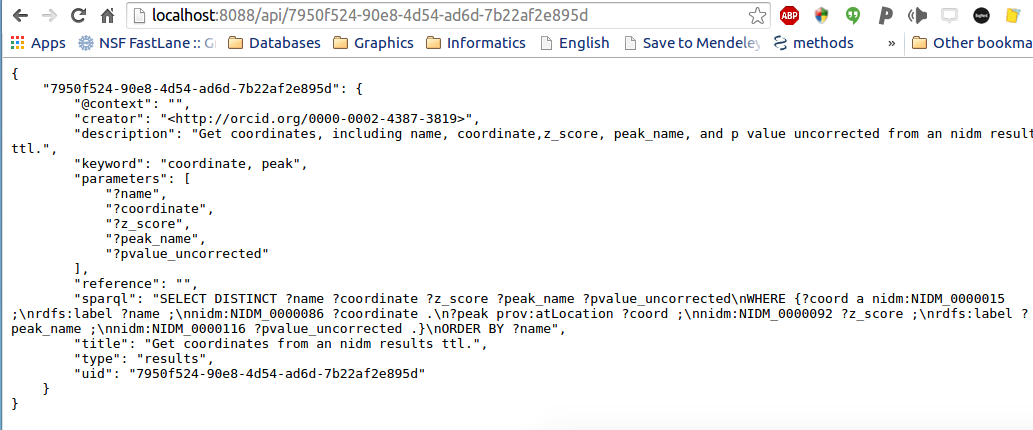
\includegraphics{singleQuery.png}

You might then have a turtle file that you want to actually run a query on. For example, if you look in the nidm-api examples directory, we have provided a nidm.ttl file that corresponds to a NIDM-Results folder. We can run the query we just saw above to get coordinates:

\begin{Verbatim}[commandchars=\\\{\}]
http://localhost:8088/api/query/7950f524\PYGZhy{}90e8\PYGZhy{}4d54\PYGZhy{}ad6d\PYGZhy{}7b22af2e895d?ttl=/home/vanessa/Desktop/nidm.ttl
\end{Verbatim}

The only difference is that we've added the ``query'' to the URL, and specified the ttl file as a variable, indicated by the ''?'' at the end of the URL. We will eventually give you more options to customize your query, for now that's it. When you do the query, your result will be returned again in json:

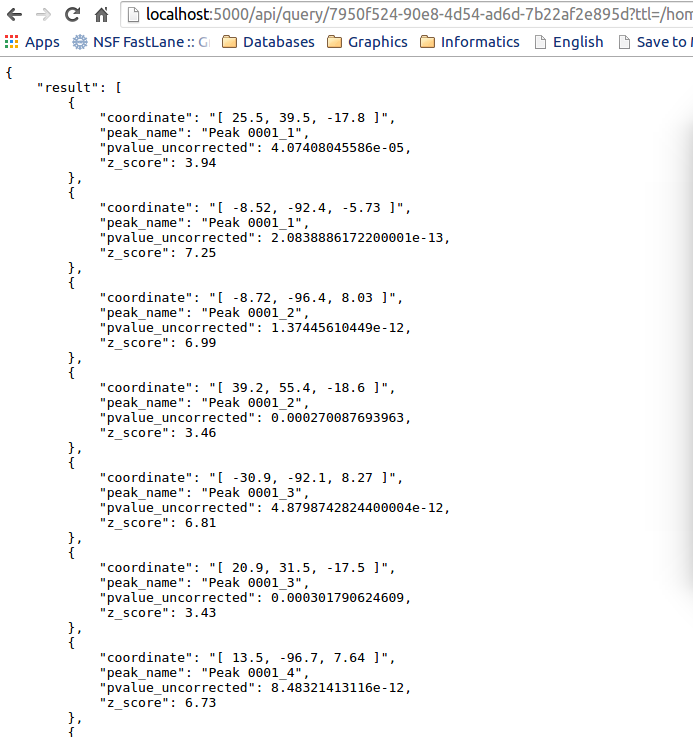
\includegraphics{doQuery.png}

Note that I gave the REST API a local path on my computer. We can also give it a URL and it will work.

\begin{Verbatim}[commandchars=\\\{\}]
http://localhost:8088/api/query/7950f524\PYGZhy{}90e8\PYGZhy{}4d54\PYGZhy{}ad6d\PYGZhy{}7b22af2e895d?ttl=https://rawgithub.com/incf\PYGZhy{}nidash/nidm\PYGZhy{}api/master/example/nidm.ttl
\end{Verbatim}

Boum.

If you screw something up, meaning that the query did not work for any reason (e.g., you gave it a wrong file, improperly formatted file, or the query logic has an error), it will tell you:

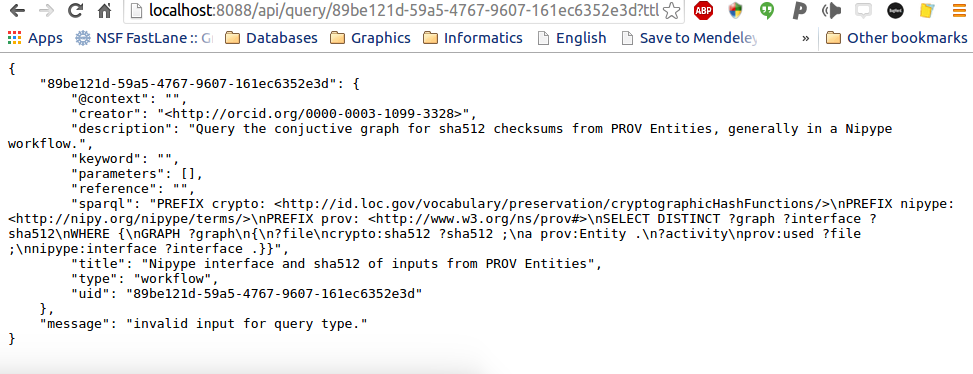
\includegraphics{screwUp.png}

Note that the current (tiny) set of queries is currently not being validated, and they need work and contribution.


\subsection{REST API on Server}
\label{getting-started:rest-api-on-server}
You can use something like gunicorn to run the flask application on a server, for the world to use. More documentation on how to do this will come, as we currently do not have a server to host this. Please be aware that the debug mode in the Flask application is set to True, and you should {\color{red}\bfseries{}{}`read about \textless{}http://flask.pocoo.org/docs/0.10/deploying/
\textgreater{}{}`\_} the proper way to deploy a flask application before doing something that might compromise the security of your server.


\subsection{Integration into Python}
\label{getting-started:integration-into-python}
An example turtle file is provided in the ``example'' directory of the repo, and running a query on this file from within python is shown below:

\begin{Verbatim}[commandchars=\\\{\}]
\PYG{c}{\PYGZsh{}!/usr/bin/python}

\PYG{k+kn}{from} \PYG{n+nn}{nidm.query} \PYG{k+kn}{import} \PYG{n}{get\PYGZus{}query\PYGZus{}directory}\PYG{p}{,} \PYG{n}{validate\PYGZus{}queries}\PYG{p}{,} \PYG{n}{make\PYGZus{}lookup}\PYG{p}{,} \PYG{n}{do\PYGZus{}query}

\PYG{c}{\PYGZsh{} Get updated queries, validate, and generate a lookup dict:}
\PYG{n}{query\PYGZus{}dir} \PYG{o}{=} \PYG{n}{get\PYGZus{}query\PYGZus{}directory}\PYG{p}{(}\PYG{p}{)}
\PYG{n}{query\PYGZus{}json} \PYG{o}{=} \PYG{n}{validate\PYGZus{}queries}\PYG{p}{(}\PYG{n}{query\PYGZus{}dir}\PYG{p}{)}
\PYG{n}{query\PYGZus{}dict} \PYG{o}{=} \PYG{n}{make\PYGZus{}lookup}\PYG{p}{(}\PYG{n}{query\PYGZus{}json}\PYG{p}{,}\PYG{n}{key\PYGZus{}field}\PYG{o}{=}\PYG{l+s}{\PYGZdq{}}\PYG{l+s}{uid}\PYG{l+s}{\PYGZdq{}}\PYG{p}{)}

\PYG{c}{\PYGZsh{} Let\PYGZsq{}s use the query to get coordinates}
\PYG{n}{qid} \PYG{o}{=} \PYG{l+s}{\PYGZdq{}}\PYG{l+s}{7950f524\PYGZhy{}90e8\PYGZhy{}4d54\PYGZhy{}ad6d\PYGZhy{}7b22af2e895d}\PYG{l+s}{\PYGZdq{}}

\PYG{c}{\PYGZsh{} Here is a ttl file that I want to query, nidm\PYGZhy{}results}
\PYG{n}{ttl\PYGZus{}file} \PYG{o}{=} \PYG{l+s}{\PYGZdq{}}\PYG{l+s}{nidm.ttl}\PYG{l+s}{\PYGZdq{}}

\PYG{n}{result} \PYG{o}{=} \PYG{n}{do\PYGZus{}query}\PYG{p}{(}\PYG{n}{ttl\PYGZus{}file}\PYG{o}{=}\PYG{n}{ttl\PYGZus{}file}\PYG{p}{,}\PYG{n}{query}\PYG{o}{=}\PYG{n}{query\PYGZus{}dict}\PYG{p}{[}\PYG{n}{qid}\PYG{p}{]}\PYG{p}{[}\PYG{l+s}{\PYGZdq{}}\PYG{l+s}{sparql}\PYG{l+s}{\PYGZdq{}}\PYG{p}{]}\PYG{p}{)}

\PYG{c}{\PYGZsh{} The result is a pandas data frame. I can turn it into other things too}
\PYG{n}{result} \PYG{o}{=} \PYG{n}{result}\PYG{o}{.}\PYG{n}{to\PYGZus{}dict}\PYG{p}{(}\PYG{n}{orient}\PYG{o}{=}\PYG{l+s}{\PYGZdq{}}\PYG{l+s}{records}\PYG{l+s}{\PYGZdq{}}\PYG{p}{)}
\end{Verbatim}


\section{nidm}
\label{modules::doc}\label{modules:nidm}

\subsection{nidm package}
\label{nidm:nidm-package}\label{nidm::doc}

\subsubsection{Subpackages}
\label{nidm:subpackages}

\paragraph{nidm.script package}
\label{nidm.script::doc}\label{nidm.script:nidm-script-package}

\subparagraph{Submodules}
\label{nidm.script:submodules}

\subparagraph{nidm.script.post\_install module}
\label{nidm.script:module-nidm.script.post_install}\label{nidm.script:nidm-script-post-install-module}\index{nidm.script.post\_install (module)}

\subparagraph{Module contents}
\label{nidm.script:module-contents}\label{nidm.script:module-nidm.script}\index{nidm.script (module)}

\paragraph{nidm.templates package}
\label{nidm.templates::doc}\label{nidm.templates:nidm-templates-package}

\subparagraph{Module contents}
\label{nidm.templates:module-contents}\label{nidm.templates:module-nidm.templates}\index{nidm.templates (module)}

\subsubsection{Submodules}
\label{nidm:submodules}

\subsubsection{nidm.app module}
\label{nidm:module-nidm.app}\label{nidm:nidm-app-module}\index{nidm.app (module)}\index{NIDMServer (class in nidm.app)}

\begin{fulllineitems}
\phantomsection\label{nidm:nidm.app.NIDMServer}\pysiglinewithargsret{\strong{class }\code{nidm.app.}\bfcode{NIDMServer}}{\emph{*args}, \emph{**kwargs}}{}
Bases: \code{flask.app.Flask}

\end{fulllineitems}

\index{apiDoQuery (class in nidm.app)}

\begin{fulllineitems}
\phantomsection\label{nidm:nidm.app.apiDoQuery}\pysigline{\strong{class }\code{nidm.app.}\bfcode{apiDoQuery}}
Bases: \code{flask\_restful.Resource}

return result of query on ttl file
Paramters
=========
qid: str
\begin{quote}

the uid associated with the query
\end{quote}
\begin{description}
\item[{ttl: str}] \leavevmode
the url of the turtle file

\end{description}
\index{endpoint (nidm.app.apiDoQuery attribute)}

\begin{fulllineitems}
\phantomsection\label{nidm:nidm.app.apiDoQuery.endpoint}\pysigline{\bfcode{endpoint}\strong{ = `apidoquery'}}
\end{fulllineitems}

\index{get() (nidm.app.apiDoQuery method)}

\begin{fulllineitems}
\phantomsection\label{nidm:nidm.app.apiDoQuery.get}\pysiglinewithargsret{\bfcode{get}}{\emph{qid}, \emph{output\_format}}{}
\end{fulllineitems}

\index{mediatypes() (nidm.app.apiDoQuery method)}

\begin{fulllineitems}
\phantomsection\label{nidm:nidm.app.apiDoQuery.mediatypes}\pysiglinewithargsret{\bfcode{mediatypes}}{\emph{resource\_cls}}{}
\end{fulllineitems}

\index{methods (nidm.app.apiDoQuery attribute)}

\begin{fulllineitems}
\phantomsection\label{nidm:nidm.app.apiDoQuery.methods}\pysigline{\bfcode{methods}\strong{ = {[}'GET'{]}}}
\end{fulllineitems}


\end{fulllineitems}

\index{apiIndex (class in nidm.app)}

\begin{fulllineitems}
\phantomsection\label{nidm:nidm.app.apiIndex}\pysigline{\strong{class }\code{nidm.app.}\bfcode{apiIndex}}
Bases: \code{flask\_restful.Resource}

Main view for REST API to display all available queries
\index{endpoint (nidm.app.apiIndex attribute)}

\begin{fulllineitems}
\phantomsection\label{nidm:nidm.app.apiIndex.endpoint}\pysigline{\bfcode{endpoint}\strong{ = `apiindex'}}
\end{fulllineitems}

\index{get() (nidm.app.apiIndex method)}

\begin{fulllineitems}
\phantomsection\label{nidm:nidm.app.apiIndex.get}\pysiglinewithargsret{\bfcode{get}}{}{}
\end{fulllineitems}

\index{mediatypes() (nidm.app.apiIndex method)}

\begin{fulllineitems}
\phantomsection\label{nidm:nidm.app.apiIndex.mediatypes}\pysiglinewithargsret{\bfcode{mediatypes}}{\emph{resource\_cls}}{}
\end{fulllineitems}

\index{methods (nidm.app.apiIndex attribute)}

\begin{fulllineitems}
\phantomsection\label{nidm:nidm.app.apiIndex.methods}\pysigline{\bfcode{methods}\strong{ = {[}'GET'{]}}}
\end{fulllineitems}


\end{fulllineitems}

\index{apiQueryMeta (class in nidm.app)}

\begin{fulllineitems}
\phantomsection\label{nidm:nidm.app.apiQueryMeta}\pysigline{\strong{class }\code{nidm.app.}\bfcode{apiQueryMeta}}
Bases: \code{flask\_restful.Resource}

return complete meta data for specific query
\index{endpoint (nidm.app.apiQueryMeta attribute)}

\begin{fulllineitems}
\phantomsection\label{nidm:nidm.app.apiQueryMeta.endpoint}\pysigline{\bfcode{endpoint}\strong{ = `apiquerymeta'}}
\end{fulllineitems}

\index{get() (nidm.app.apiQueryMeta method)}

\begin{fulllineitems}
\phantomsection\label{nidm:nidm.app.apiQueryMeta.get}\pysiglinewithargsret{\bfcode{get}}{\emph{qid}}{}
\end{fulllineitems}

\index{mediatypes() (nidm.app.apiQueryMeta method)}

\begin{fulllineitems}
\phantomsection\label{nidm:nidm.app.apiQueryMeta.mediatypes}\pysiglinewithargsret{\bfcode{mediatypes}}{\emph{resource\_cls}}{}
\end{fulllineitems}

\index{methods (nidm.app.apiQueryMeta attribute)}

\begin{fulllineitems}
\phantomsection\label{nidm:nidm.app.apiQueryMeta.methods}\pysigline{\bfcode{methods}\strong{ = {[}'GET'{]}}}
\end{fulllineitems}


\end{fulllineitems}

\index{start() (in module nidm.app)}

\begin{fulllineitems}
\phantomsection\label{nidm:nidm.app.start}\pysiglinewithargsret{\code{nidm.app.}\bfcode{start}}{\emph{port=8088}}{}
\end{fulllineitems}



\subsubsection{nidm.experiment module}
\label{nidm:module-nidm.experiment}\label{nidm:nidm-experiment-module}\index{nidm.experiment (module)}
experiment: part of the nidm-api
functions for working with nidm experiment


\subsubsection{nidm.query module}
\label{nidm:module-nidm.query}\label{nidm:nidm-query-module}\index{nidm.query (module)}
query: part of the nidm-api
general functions to work with query
data structures for nidm-queries
\index{do\_query() (in module nidm.query)}

\begin{fulllineitems}
\phantomsection\label{nidm:nidm.query.do_query}\pysiglinewithargsret{\code{nidm.query.}\bfcode{do\_query}}{\emph{ttl\_file}, \emph{query}, \emph{rdf\_format='turtle'}, \emph{serialize\_format='csv'}, \emph{output\_df=True}}{}
\end{fulllineitems}

\index{download\_queries() (in module nidm.query)}

\begin{fulllineitems}
\phantomsection\label{nidm:nidm.query.download_queries}\pysiglinewithargsret{\code{nidm.query.}\bfcode{download\_queries}}{\emph{destination}}{}
Download queries repo to a destination
Parameters
==========
destination:
\begin{quote}

the full path to download the repo to
\end{quote}

\end{fulllineitems}

\index{find\_queries() (in module nidm.query)}

\begin{fulllineitems}
\phantomsection\label{nidm:nidm.query.find_queries}\pysiglinewithargsret{\code{nidm.query.}\bfcode{find\_queries}}{\emph{query\_folders}, \emph{search\_pattern='*.json'}}{}
searches one or more folders for valid queries, meaning
json files. In the case of multiple directories, will
append the folder name as a variable to indicate the type
Parameters
==========
query\_folders: list or str
\begin{quote}

one or more full paths to directories with json objects
\end{quote}
\begin{description}
\item[{search\_pattern: str}] \leavevmode
pattern for glob to use to find query objects
default is ``{\color{red}\bfseries{}*}.json''

\end{description}
\begin{description}
\item[{queries: list}] \leavevmode
a list of full paths to query object files

\end{description}

\end{fulllineitems}

\index{generate\_query\_template() (in module nidm.query)}

\begin{fulllineitems}
\phantomsection\label{nidm:nidm.query.generate_query_template}\pysiglinewithargsret{\code{nidm.query.}\bfcode{generate\_query\_template}}{\emph{output\_dir=None}, \emph{template\_path=None}, \emph{fields=None}}{}~\begin{description}
\item[{output\_dir: str}] \leavevmode
full path to output directory for json data structure.
if none specified, will not save the data structure

\item[{template\_path: str}] \leavevmode
path to json file to use as a template. Only should be
specified if the user has reason to use a custom template
default is the standard provided by nidm-api.

\item[{fields: dict (optional)}] \leavevmode
a dictionary with fields that correspond to template keys.
if provided, template will be filled with keys. Possible values
include

\end{description}
\begin{description}
\item[{template: json (dict)}] \leavevmode
A python dictionary (json) that can be filled with
new query information

\end{description}

\end{fulllineitems}

\index{get\_query\_directory() (in module nidm.query)}

\begin{fulllineitems}
\phantomsection\label{nidm:nidm.query.get_query_directory}\pysiglinewithargsret{\code{nidm.query.}\bfcode{get\_query\_directory}}{\emph{tmpdir=None}}{}
get\_query\_directory:
Download queries repo to tmp directory
Parameters
==========
tmpdir: str
\begin{quote}

path to directory to download queries to
\end{quote}

\end{fulllineitems}

\index{make\_lookup() (in module nidm.query)}

\begin{fulllineitems}
\phantomsection\label{nidm:nidm.query.make_lookup}\pysiglinewithargsret{\code{nidm.query.}\bfcode{make\_lookup}}{\emph{query\_list}, \emph{key\_field}}{}
returns dict object to quickly look up query based on uid
Parameters
==========
query\_list: list
\begin{quote}

a list of query (dict objects)
\end{quote}
\begin{description}
\item[{key\_field: str}] \leavevmode
the key in the dictionary to base the lookup key

\end{description}
\begin{description}
\item[{query\_dict: dict}] \leavevmode
dict (json) with key as ``key\_field'' from query\_list

\end{description}

\end{fulllineitems}

\index{read\_queries() (in module nidm.query)}

\begin{fulllineitems}
\phantomsection\label{nidm:nidm.query.read_queries}\pysiglinewithargsret{\code{nidm.query.}\bfcode{read\_queries}}{\emph{query\_paths}}{}
Read in a list of query (json) objects.
Parameters
==========
query\_paths: list
a list of full paths to query objects to read
Returns
=======
{\color{red}\bfseries{}queries\_}: list
\begin{quote}

dict to be served as json describing queries available
a ``type'' variable is added to indicate folder query was found in
\end{quote}

\end{fulllineitems}

\index{save\_query\_template() (in module nidm.query)}

\begin{fulllineitems}
\phantomsection\label{nidm:nidm.query.save_query_template}\pysiglinewithargsret{\code{nidm.query.}\bfcode{save\_query\_template}}{\emph{template}, \emph{output\_dir}}{}
generate\_query\_template
Parameters
==========
output\_dir: string path
\begin{quote}

full path to output directory for json data structure.
the template filename is generated from the uid variable
\end{quote}
\begin{description}
\item[{success: boolean}] \leavevmode
True if save was successful, false otherwise

\end{description}

\end{fulllineitems}

\index{validate\_queries() (in module nidm.query)}

\begin{fulllineitems}
\phantomsection\label{nidm:nidm.query.validate_queries}\pysiglinewithargsret{\code{nidm.query.}\bfcode{validate\_queries}}{\emph{query\_dir}, \emph{queries=None}}{}
returns json object with query data structures, and
a field `valid' to describe if query was valid
Parameters
==========
queries: list
\begin{quote}

a list of full paths to json files, each a query
\end{quote}
\begin{description}
\item[{query\_dir: str}] \leavevmode
full path to a nidm-query repo

\end{description}
\begin{description}
\item[{queries: json}] \leavevmode
dict (json) with all read in queries available

\end{description}

from nidm-query, provided by API

\end{fulllineitems}



\subsubsection{nidm.results module}
\label{nidm:module-nidm.results}\label{nidm:nidm-results-module}\index{nidm.results (module)}
results: part of the nidm-api
functions for working with nidm results


\subsubsection{nidm.scripts module}
\label{nidm:module-nidm.scripts}\label{nidm:nidm-scripts-module}\index{nidm.scripts (module)}
script.py: part of nidmapi package
Runtime executable
\index{main() (in module nidm.scripts)}

\begin{fulllineitems}
\phantomsection\label{nidm:nidm.scripts.main}\pysiglinewithargsret{\code{nidm.scripts.}\bfcode{main}}{}{}
\end{fulllineitems}



\subsubsection{nidm.utils module}
\label{nidm:module-nidm.utils}\label{nidm:nidm-utils-module}\index{nidm.utils (module)}
utils: part of the nidm-api
general functions for the api
\index{clean\_fields() (in module nidm.utils)}

\begin{fulllineitems}
\phantomsection\label{nidm:nidm.utils.clean_fields}\pysiglinewithargsret{\code{nidm.utils.}\bfcode{clean\_fields}}{\emph{mydict}}{}
Ensures that keys and values of dictionary are in utf-8
so rendering in javascript is clean.
Paramters
=========
mydict: dict
\begin{quote}

dictionary to clean
\end{quote}
\begin{description}
\item[{newdict: dict}] \leavevmode
dictionary with all fields encoded in utf-8

\end{description}

\end{fulllineitems}

\index{copy\_directory() (in module nidm.utils)}

\begin{fulllineitems}
\phantomsection\label{nidm:nidm.utils.copy_directory}\pysiglinewithargsret{\code{nidm.utils.}\bfcode{copy\_directory}}{\emph{src}, \emph{dest}}{}
Copy an entire directory recursively

\end{fulllineitems}

\index{find\_directories() (in module nidm.utils)}

\begin{fulllineitems}
\phantomsection\label{nidm:nidm.utils.find_directories}\pysiglinewithargsret{\code{nidm.utils.}\bfcode{find\_directories}}{\emph{root}, \emph{fullpath=True}}{}
Return directories at one level specified by user
(not recursive)

\end{fulllineitems}

\index{find\_subdirectories() (in module nidm.utils)}

\begin{fulllineitems}
\phantomsection\label{nidm:nidm.utils.find_subdirectories}\pysiglinewithargsret{\code{nidm.utils.}\bfcode{find\_subdirectories}}{\emph{basepath}}{}
Return directories (and sub) starting from a base

\end{fulllineitems}

\index{get\_installdir() (in module nidm.utils)}

\begin{fulllineitems}
\phantomsection\label{nidm:nidm.utils.get_installdir}\pysiglinewithargsret{\code{nidm.utils.}\bfcode{get\_installdir}}{}{}
returns installation directory of nidm-api

\end{fulllineitems}

\index{get\_query\_template() (in module nidm.utils)}

\begin{fulllineitems}
\phantomsection\label{nidm:nidm.utils.get_query_template}\pysiglinewithargsret{\code{nidm.utils.}\bfcode{get\_query\_template}}{}{}
get\_standard\_template
returns the full path to the standard template for queries

\end{fulllineitems}

\index{get\_template() (in module nidm.utils)}

\begin{fulllineitems}
\phantomsection\label{nidm:nidm.utils.get_template}\pysiglinewithargsret{\code{nidm.utils.}\bfcode{get\_template}}{\emph{template\_file}}{}
get\_template: read in and return a template file

\end{fulllineitems}

\index{has\_internet\_connectivity() (in module nidm.utils)}

\begin{fulllineitems}
\phantomsection\label{nidm:nidm.utils.has_internet_connectivity}\pysiglinewithargsret{\code{nidm.utils.}\bfcode{has\_internet\_connectivity}}{}{}
Checks for internet connectivity by way of trying to
retrieve google IP address. Returns True/False

\end{fulllineitems}

\index{is\_type() (in module nidm.utils)}

\begin{fulllineitems}
\phantomsection\label{nidm:nidm.utils.is_type}\pysiglinewithargsret{\code{nidm.utils.}\bfcode{is\_type}}{\emph{var, types={[}\textless{}type `int'\textgreater{}, \textless{}type `float'\textgreater{}, \textless{}type `list'\textgreater{}{]}}}{}
Check type

\end{fulllineitems}

\index{load\_json() (in module nidm.utils)}

\begin{fulllineitems}
\phantomsection\label{nidm:nidm.utils.load_json}\pysiglinewithargsret{\code{nidm.utils.}\bfcode{load\_json}}{\emph{json\_path}}{}
returns a loaded json file
Parameters
==========
json\_path: str
\begin{quote}

full path to json file to load
\end{quote}
\begin{description}
\item[{thejson: json (dict)}] \leavevmode
loaded json (dict)

\end{description}

\end{fulllineitems}

\index{remove\_unicode\_dict() (in module nidm.utils)}

\begin{fulllineitems}
\phantomsection\label{nidm:nidm.utils.remove_unicode_dict}\pysiglinewithargsret{\code{nidm.utils.}\bfcode{remove\_unicode\_dict}}{\emph{input\_dict}, \emph{encoding='utf-8'}}{}
remove unicode keys and values from dict, encoding in utf8

\end{fulllineitems}

\index{save\_template() (in module nidm.utils)}

\begin{fulllineitems}
\phantomsection\label{nidm:nidm.utils.save_template}\pysiglinewithargsret{\code{nidm.utils.}\bfcode{save\_template}}{\emph{output\_file}, \emph{html\_snippet}}{}
\end{fulllineitems}

\index{set\_permissions() (in module nidm.utils)}

\begin{fulllineitems}
\phantomsection\label{nidm:nidm.utils.set_permissions}\pysiglinewithargsret{\code{nidm.utils.}\bfcode{set\_permissions}}{\emph{path}, \emph{permission=128}}{}
\end{fulllineitems}

\index{sub\_template() (in module nidm.utils)}

\begin{fulllineitems}
\phantomsection\label{nidm:nidm.utils.sub_template}\pysiglinewithargsret{\code{nidm.utils.}\bfcode{sub\_template}}{\emph{template}, \emph{template\_tag}, \emph{substitution}}{}
make a substitution for a template\_tag in a template

\end{fulllineitems}



\subsubsection{nidm.workflow module}
\label{nidm:nidm-workflow-module}\label{nidm:module-nidm.workflow}\index{nidm.workflow (module)}
workflow: part of the nidm-api
functions for working with nidm workflow


\subsubsection{Module contents}
\label{nidm:module-nidm}\label{nidm:module-contents}\index{nidm (module)}

\section{Development}
\label{development:development}\label{development::doc}

\subsection{How do I contribute a new query?}
\label{development:how-do-i-contribute-a-new-query}
We have a dynamic web interface that will allow you to generate, preview (and eventually test) a new data structure for adding to \href{https://github.com/incf-nidash/nidm-query}{nidm-query}. This can also be done, using the same functions, programatically. You can then add it to the repo by submitting a pull request to add it. A pull request affords group discussion, and we will eventually have continuous integration that will run tests on your new query. We recommend that you use the generation functions to ensure accuracy in the format and fields of your data structure.


\subsubsection{Web Query Generator}
\label{development:web-query-generator}
To generate a query with the interactive web interface, first start up the nidm application

\begin{Verbatim}[commandchars=\\\{\}]
\PYG{n}{nidm}
\end{Verbatim}

Then open your browser to localhost:8088/query/new. You will be presented with fields to fill in for your query:

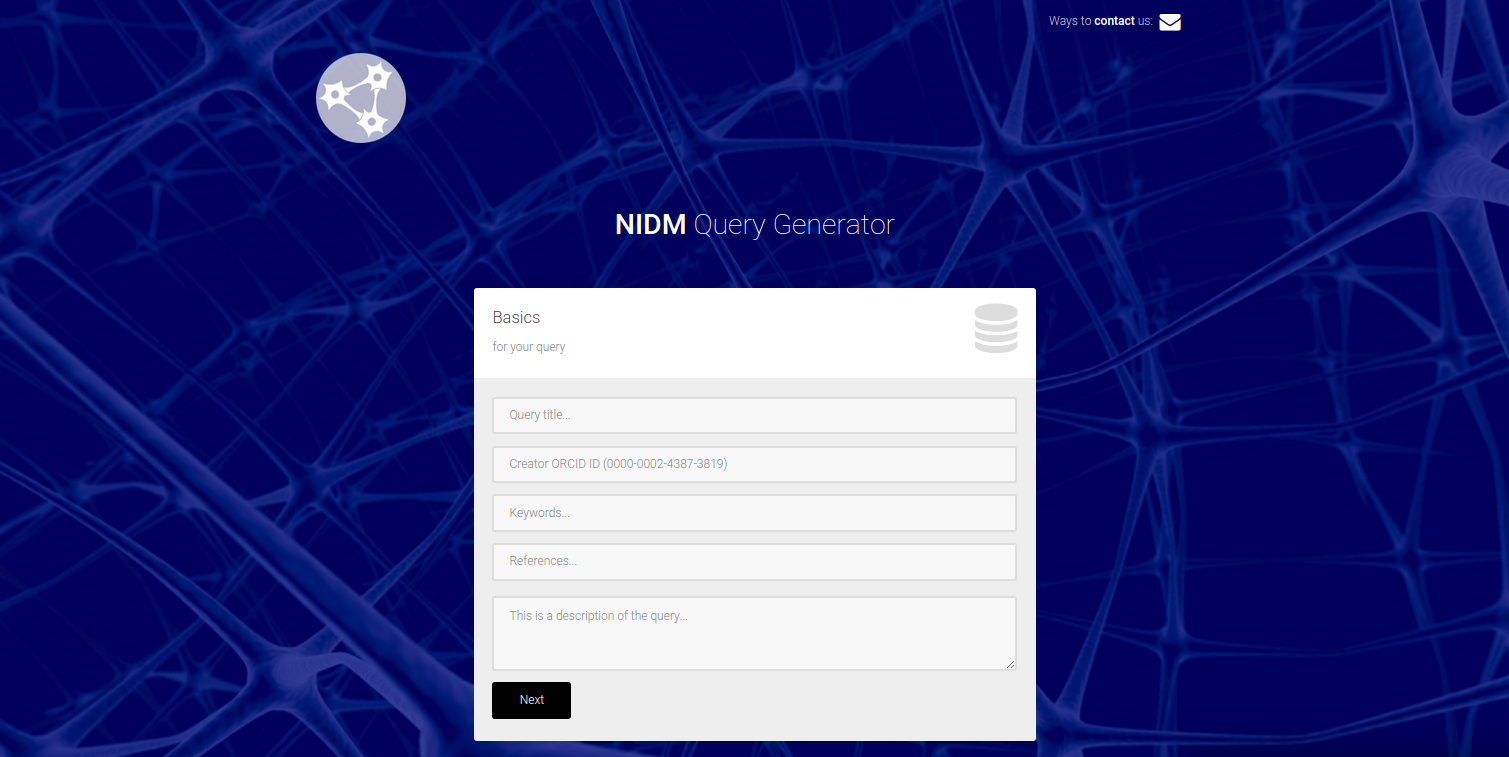
\includegraphics{queryField.png}
\begin{itemize}
\item {} 
title: This should be a single sentence that describes what your query does, what object model it is associated with, etc.

\item {} 
creator: We ask for your ORCID ID to be filled into the creator spot. If you don't have this, you can put a name or email. We are currently not validating this, so you can really do whatever you like. We will (hopefully) decide on a standard.

\item {} 
description: This should be a text description of your query, please give details. The title and description will eventually be provided in a static web interface served with the repo for people to search and find queries they want to use.

\end{itemize}

When you click next, the next page is where you should copy paste your sparql:

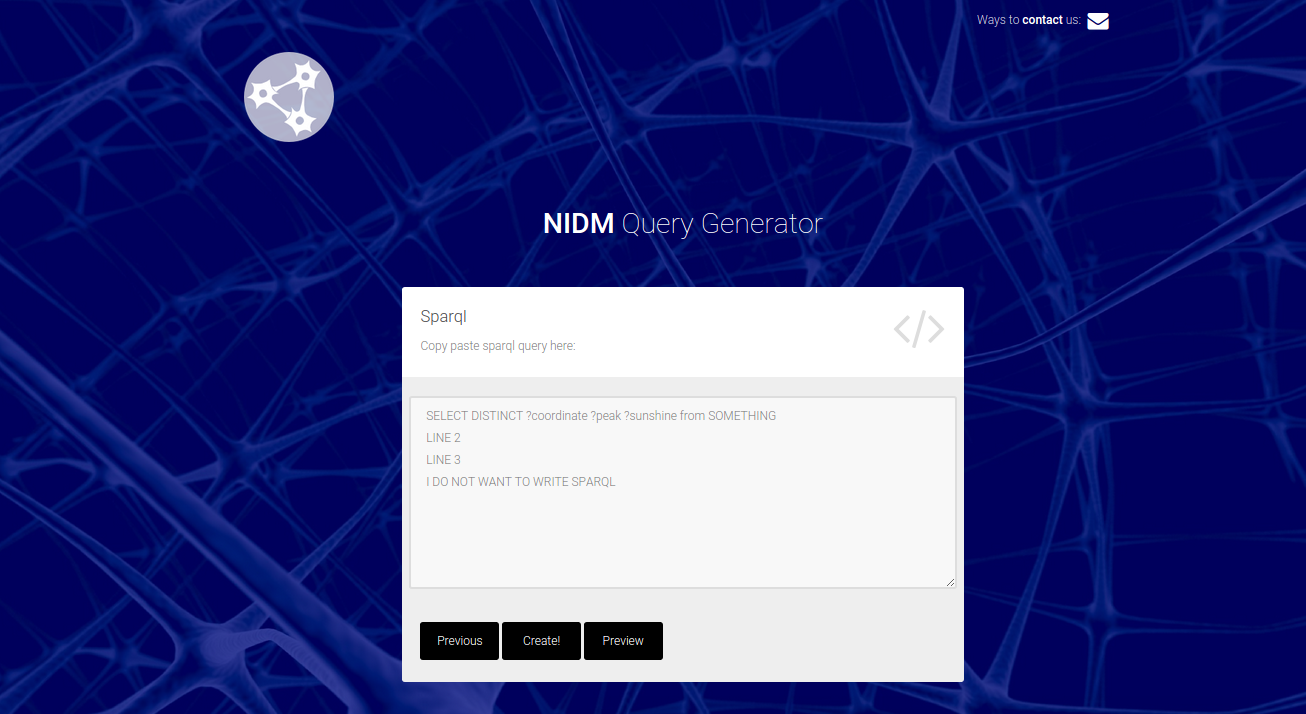
\includegraphics{querySparql.png}

If you are not ready to generate your file, you can click ``Preview'' for a new tab to open with the query. The parameters that the user is allowed to ask for will be extracted from your ``select'' line, indicated by a word preceded with ? (e.g., ?hello). Do not worry about capitalization.

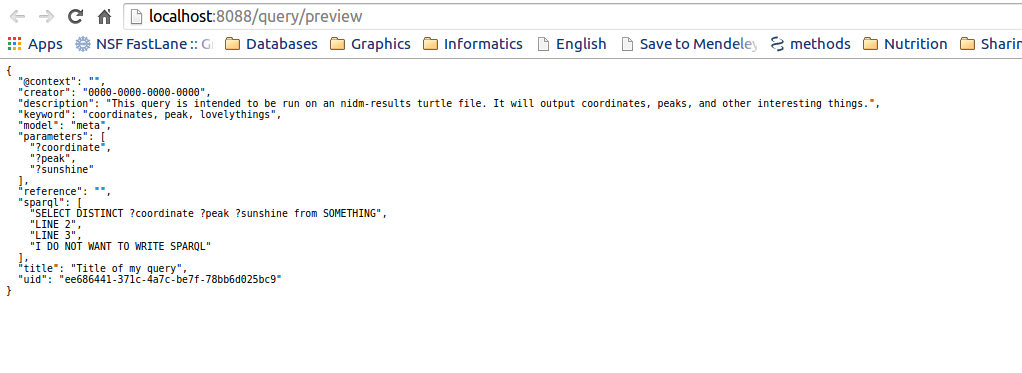
\includegraphics{queryPreview.png}

When you are ready to save your query, click ``Create!''

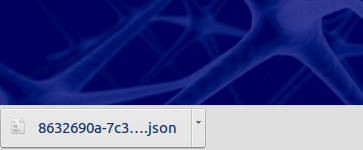
\includegraphics{queryDownload1.png}

A file will be downloaded to your computer. You should drop this file into the appropriate directory in your \href{https://github.com/incf-nidash/nidm-query}{nidm-query}. repo and submit a PR to add it to the nidm-api. We will eventually have tests for the queries, and an interactive web interface hosted with the nidm-api to explore the queries available (before downloading the nidm-api).

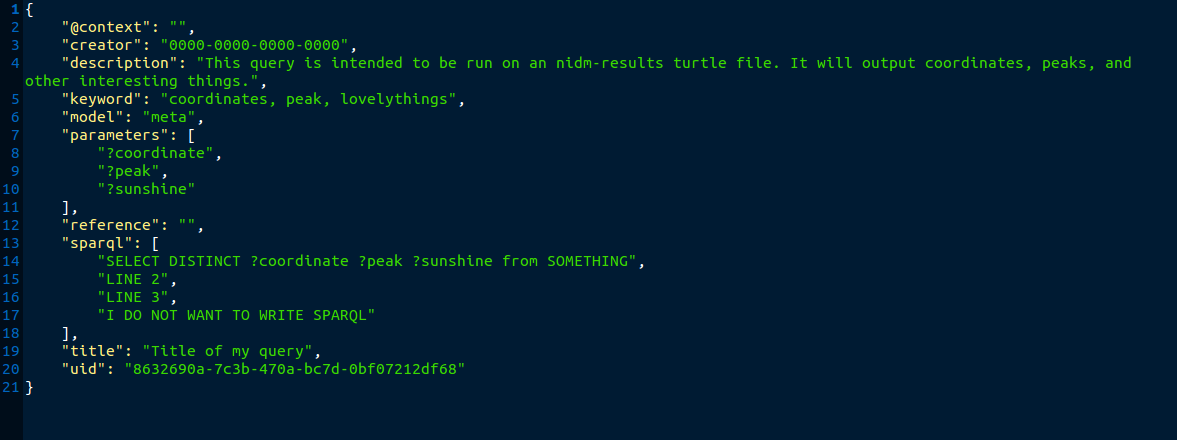
\includegraphics{queryDownload2.png}

You can then download to your local machine:


\subsection{How do I develop the API?}
\label{development:how-do-i-develop-the-api}
You will want to fork the repo, clone the fork, and then run the flask application directly (so that it updates with changes to your code):

\begin{Verbatim}[commandchars=\\\{\}]
git clone https://github.com/[username]/nidm\PYGZhy{}api
cd nidm\PYGZhy{}api
python setup.py install \PYGZhy{}\PYGZhy{}user
python nidm/app.py
\end{Verbatim}


\subsection{How does this work?}
\label{development:how-does-this-work}
Flask is a web framework (in python) that makes it ridiculously easy to do stuff with python in the browser. You can conceptually think of it like \href{https://www.djangoproject.com/}{Django} released wild and free from its mom's minivan. If you look at app.py, you will see a bunch of functions that return different views, and each view is associated with a particular url (with variables) that the user might want.  You should first familiarize yourself with flask before trying to develop with it.


\subsubsection{Queries vs. API}
\label{development:queries-vs-api}
The queries are kept separate from the api itself, in the \href{https://github.com/incf-nidash/nidm-query}{nidm-query} repo. We did this because the world of writing sparql, and developing a web framework / API to serve the queries, are two separate things. A developer writing queries should be able to submit a PR to add a single file to the nidm-queries repo without needing to know about the nidm-api infrastructure. A developer working on the API shouldn't need to worry about the sparql side of things.


\subsubsection{Application Logic}
\label{development:application-logic}
The basic application logic is as follows:
\begin{itemize}
\item {} 
The user installs the application with pip. This installs the python modules to the user's site-packages, but it also adds an executable, ``nidm'' to the users bin. This exectuable can be run to start the server instantly.

\item {} 
Upon the creation of the server, the nidm-queries repo is downloaded to a temporary directory. This ensures that queries are up to date at the start of the server. If you are using the functions from within your application, you can download the repo to a location of your choice and specify the location in your application.

\item {} 
The queries are json (ld) files. This just means they have a key called @context with some kind of stuff that semantic web folk understand. We are showing them as standard .json files because the .jsonld extension is not widely known, and could be confusing.

\item {} 
The tool reads in all queries, and presents valid queries to the user at the base url of the server, localhost:8088. (Note that validation is not currently implemented). The user can select a query of choice based on the unique id, the ``uid'' variable in the json structure presented at localhost:8088.

\item {} 
The user can then look at the details for a query by way of locahost:8088/api/{[}qid{]}, or perform a query on a ttl file with localhost:8088/api/query/{[}qid{]}?ttl={[}ttl\_file{]}. The {[}ttl\_file{]} can be a local path, or a URL. This is the extent of the tool thus far, it is still under development.

\end{itemize}


\subsection{Serving an API and web interfaces}
\label{development:serving-an-api-and-web-interfaces}
The url /api/{[}more-stuff-here{]} is linked up to serve a RESTful API, however the beauty of flask is that we can configure other URLs to do other interesting things. For example, /create might bring up an interactive web interface to write inputs to generate a new query object. /api/visual may be configured to return an interactive d3 or neo4j version of some part of the graph extracted from your ttl file. Having python and the infinite amount of web visualization technology at our fingertips makes the options really unlimited.


\chapter{Indices and tables}
\label{index:indices-and-tables}\begin{itemize}
\item {} 
\DUspan{xref,std,std-ref}{genindex}

\item {} 
\DUspan{xref,std,std-ref}{modindex}

\item {} 
\DUspan{xref,std,std-ref}{search}

\end{itemize}


\renewcommand{\indexname}{Python Module Index}
\begin{theindex}
\def\bigletter#1{{\Large\sffamily#1}\nopagebreak\vspace{1mm}}
\bigletter{n}
\item {\texttt{nidm}}, \pageref{nidm:module-nidm}
\item {\texttt{nidm.app}}, \pageref{nidm:module-nidm.app}
\item {\texttt{nidm.experiment}}, \pageref{nidm:module-nidm.experiment}
\item {\texttt{nidm.query}}, \pageref{nidm:module-nidm.query}
\item {\texttt{nidm.results}}, \pageref{nidm:module-nidm.results}
\item {\texttt{nidm.script}}, \pageref{nidm.script:module-nidm.script}
\item {\texttt{nidm.script.post\_install}}, \pageref{nidm.script:module-nidm.script.post_install}
\item {\texttt{nidm.scripts}}, \pageref{nidm:module-nidm.scripts}
\item {\texttt{nidm.templates}}, \pageref{nidm.templates:module-nidm.templates}
\item {\texttt{nidm.utils}}, \pageref{nidm:module-nidm.utils}
\item {\texttt{nidm.workflow}}, \pageref{nidm:module-nidm.workflow}
\end{theindex}

\renewcommand{\indexname}{Index}
\printindex
\end{document}
